% Diagram 2/3 — Object storage: three buckets by access tier
% Structure follows apps/api/README.md.  Workflow -> workflow.tex · DB -> database.tex
% Build:  pdflatex storage.tex
\documentclass[border=14pt]{standalone}
\usepackage[T1]{fontenc}
\usepackage{lmodern}
\usepackage{tikz}
\usetikzlibrary{positioning, arrows.meta, backgrounds, fit, calc}

\definecolor{privRed}{HTML}{B23A48}
\definecolor{privBg}{HTML}{F7E6E8}
\definecolor{signAmber}{HTML}{B7791F}
\definecolor{signBg}{HTML}{FBF1DA}
\definecolor{pubGreen}{HTML}{2E7D32}
\definecolor{pubBg}{HTML}{E6F4E6}
\definecolor{inkGray}{HTML}{475569}
\definecolor{todoGray}{HTML}{6B7280}

\newcommand{\fo}[1]{\textbf{\ttfamily #1}}                                   % folder
\newcommand{\fl}[1]{{\ttfamily\textcolor{inkGray}{#1}}}                      % leaf file
\newcommand{\an}[1]{{\scriptsize\itshape\textcolor{todoGray}{#1}}}           % annotation
\newcommand{\cpt}[1]{{\footnotesize\itshape\textcolor{inkGray}{#1}}}         % caption

\begin{document}
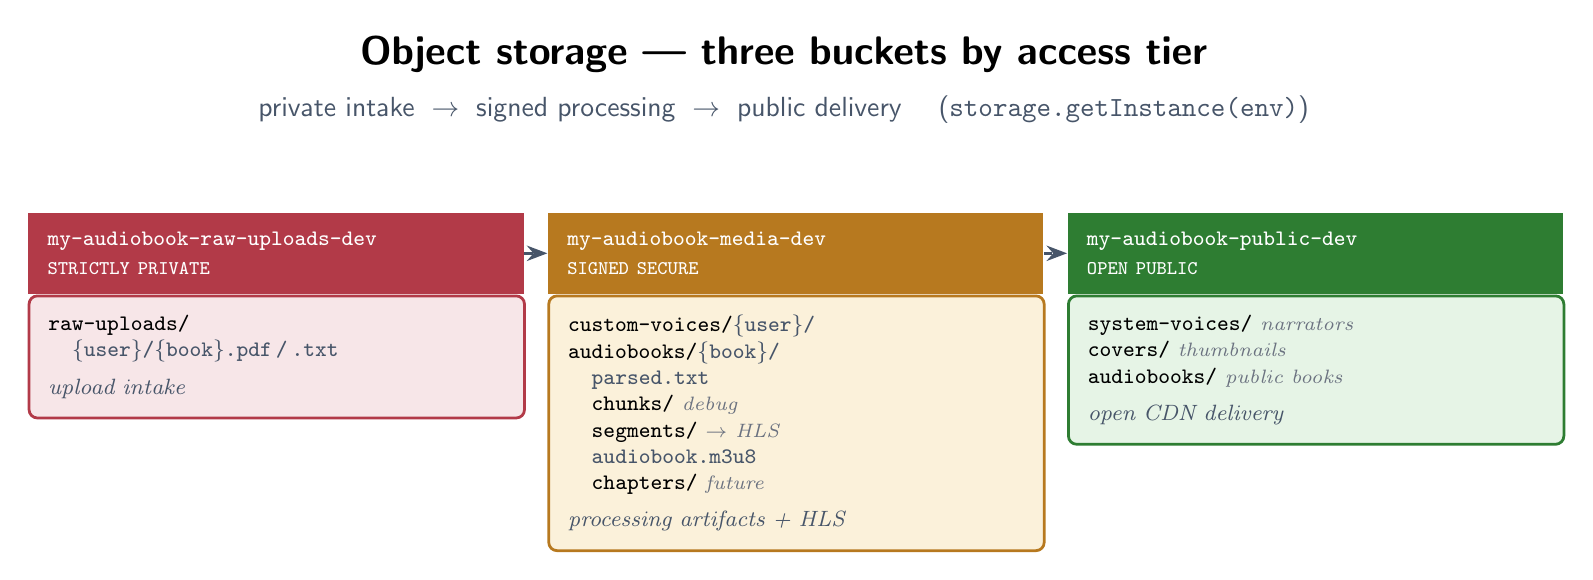
\begin{tikzpicture}[
  font=\sffamily,
  >={Stealth[length=2.6mm]},
  hbar/.style={rectangle, text=white, align=left, inner sep=7pt, text width=58mm, font=\footnotesize},
  card/.style={rectangle, rounded corners=3pt, line width=1pt, align=left,
               inner sep=7pt, text width=58mm, font=\footnotesize},
  hop/.style={->, line width=1pt, draw=inkGray, dashed},
]

% ===== Title ================================================================
\node[font=\sffamily\bfseries\Large] (title) at (9.6,2.0) {Object storage — three buckets by access tier};
\node[below=0.5mm of title, font=\sffamily, text=inkGray]
  {private intake \;$\to$\; signed processing \;$\to$\; public delivery \quad(\texttt{storage.getInstance(env)})};

% ===== 1) RAW — private intake =============================================
\node[hbar, fill=privRed, anchor=north west] (rawh) at (0,0)
  {\ttfamily\bfseries my-audiobook-raw-uploads-dev\\[1pt] \scriptsize STRICTLY PRIVATE};
\node[card, fill=privBg, draw=privRed, anchor=north west] (rawb) at (rawh.south west)
  {\fo{raw-uploads/}\\
   \hspace*{3mm}\fl{\{user\}/\{book\}.pdf\,/\,.txt}\\[4pt]
   \cpt{upload intake}};

% ===== 2) MEDIA — signed processing ========================================
\node[hbar, fill=signAmber, anchor=north west] (medh) at (6.6,0)
  {\ttfamily\bfseries my-audiobook-media-dev\\[1pt] \scriptsize SIGNED SECURE};
\node[card, fill=signBg, draw=signAmber, anchor=north west] (medb) at (medh.south west)
  {\fo{custom-voices/}\fl{\{user\}/}\\
   \fo{audiobooks/}\fl{\{book\}/}\\
   \hspace*{3mm}\fl{parsed.txt}\\
   \hspace*{3mm}\fo{chunks/} \an{debug}\\
   \hspace*{3mm}\fo{segments/} \an{$\to$ HLS}\\
   \hspace*{3mm}\fl{audiobook.m3u8}\\
   \hspace*{3mm}\fo{chapters/} \an{future}\\[4pt]
   \cpt{processing artifacts + HLS}};

% ===== 3) PUBLIC — public delivery =========================================
\node[hbar, fill=pubGreen, anchor=north west] (pubh) at (13.2,0)
  {\ttfamily\bfseries my-audiobook-public-dev\\[1pt] \scriptsize OPEN PUBLIC};
\node[card, fill=pubBg, draw=pubGreen, anchor=north west] (pubb) at (pubh.south west)
  {\fo{system-voices/} \an{narrators}\\
   \fo{covers/} \an{thumbnails}\\
   \fo{audiobooks/} \an{public books}\\[4pt]
   \cpt{open CDN delivery}};

% ===== tier-flow arrows =====================================================
\draw[hop] (rawh.east) -- (medh.west);
\draw[hop] (medh.east) -- (pubh.west);

\end{tikzpicture}
\end{document}
